The telecommunication company Nett provides capacity between cites in Europe. The cities are Stockholm, Berlin, London, Warsaw, Paris, Madrid and Rome. Some of the cities are connected in which traffic can be sent in both directions. The connections and the maximum traffic which can be sent between the cites respectively can be seen in Figure 1.

Nett wishes to provide 50 Gbit/s between Stockholm and Rome at the same time they provide 40 Gbit/s between London and Warsaw. They need help in routing the traffic because of the capacity limitations. Also, they would like to investigate if there is any slack in the network, potential to adding another traffic route and how to handle fluctuations in capacity.

\begin{center}
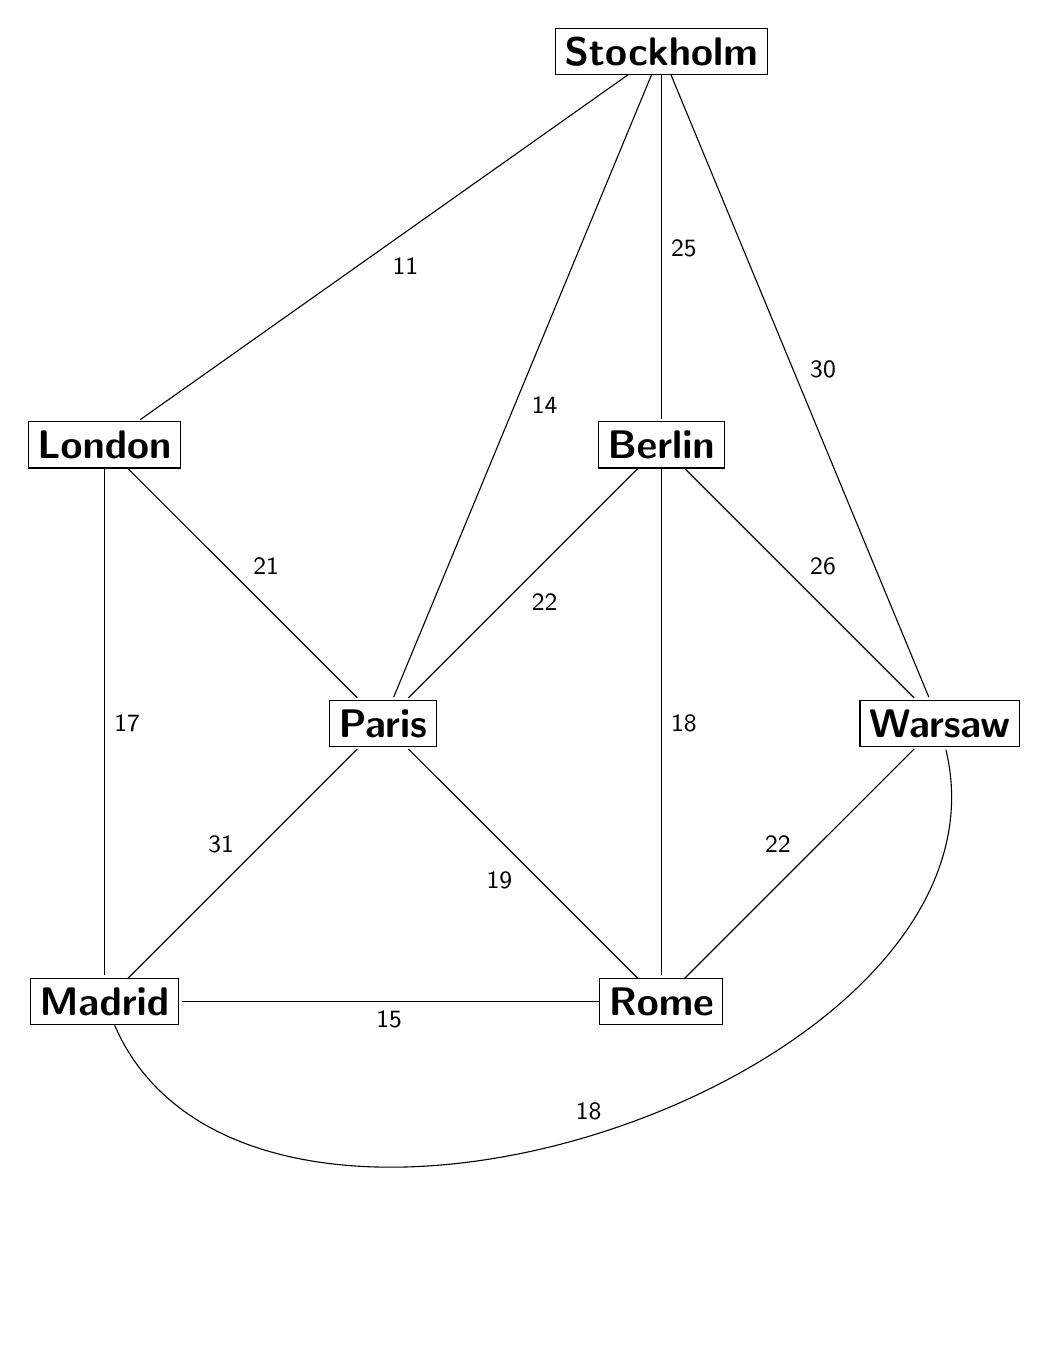
\begin{tikzpicture}[shorten >=1pt,auto,node distance=5cm,
                    main node/.style={rectangle,draw,font=\sffamily\Large\bfseries}]
  \node[main node] (1) {Stockholm};
  \node[main node] (2) [below of=1] {Berlin};
  \node[main node] (3) [below right of=2] {Warsaw};
  \node[main node] (4) [below left of=2] {Paris};
  \node[main node] (5) [above left of=4] {London};
  \node[main node] (6) [below right of=4] {Rome};
  \node[main node] (7) [below left of=4] {Madrid};

  \path[every node/.style={font=\sffamily\small}]
    (1) edge node {25} (2)
     	edge node {30} (3)
    	edge node {14} (4)
    	edge node {11} (5)
    (2) edge node {26} (3)
    	edge node {22} (4)
        edge node {18} (6)
    (5) edge node {17} (7)
        edge node {21} (4)
    (6) edge node {19} (4)
        edge node {15} (7)
        edge node {22} (3)
    (7) edge [bend right=85] node {18} (3)
    	edge node {31} (4);
  
\end{tikzpicture}
\end{center}
Figure 1. System modelled as a network where maximum capacity is marked out on the arcs.

\newpage

\section*{Routing the traffic}

\begin{center}
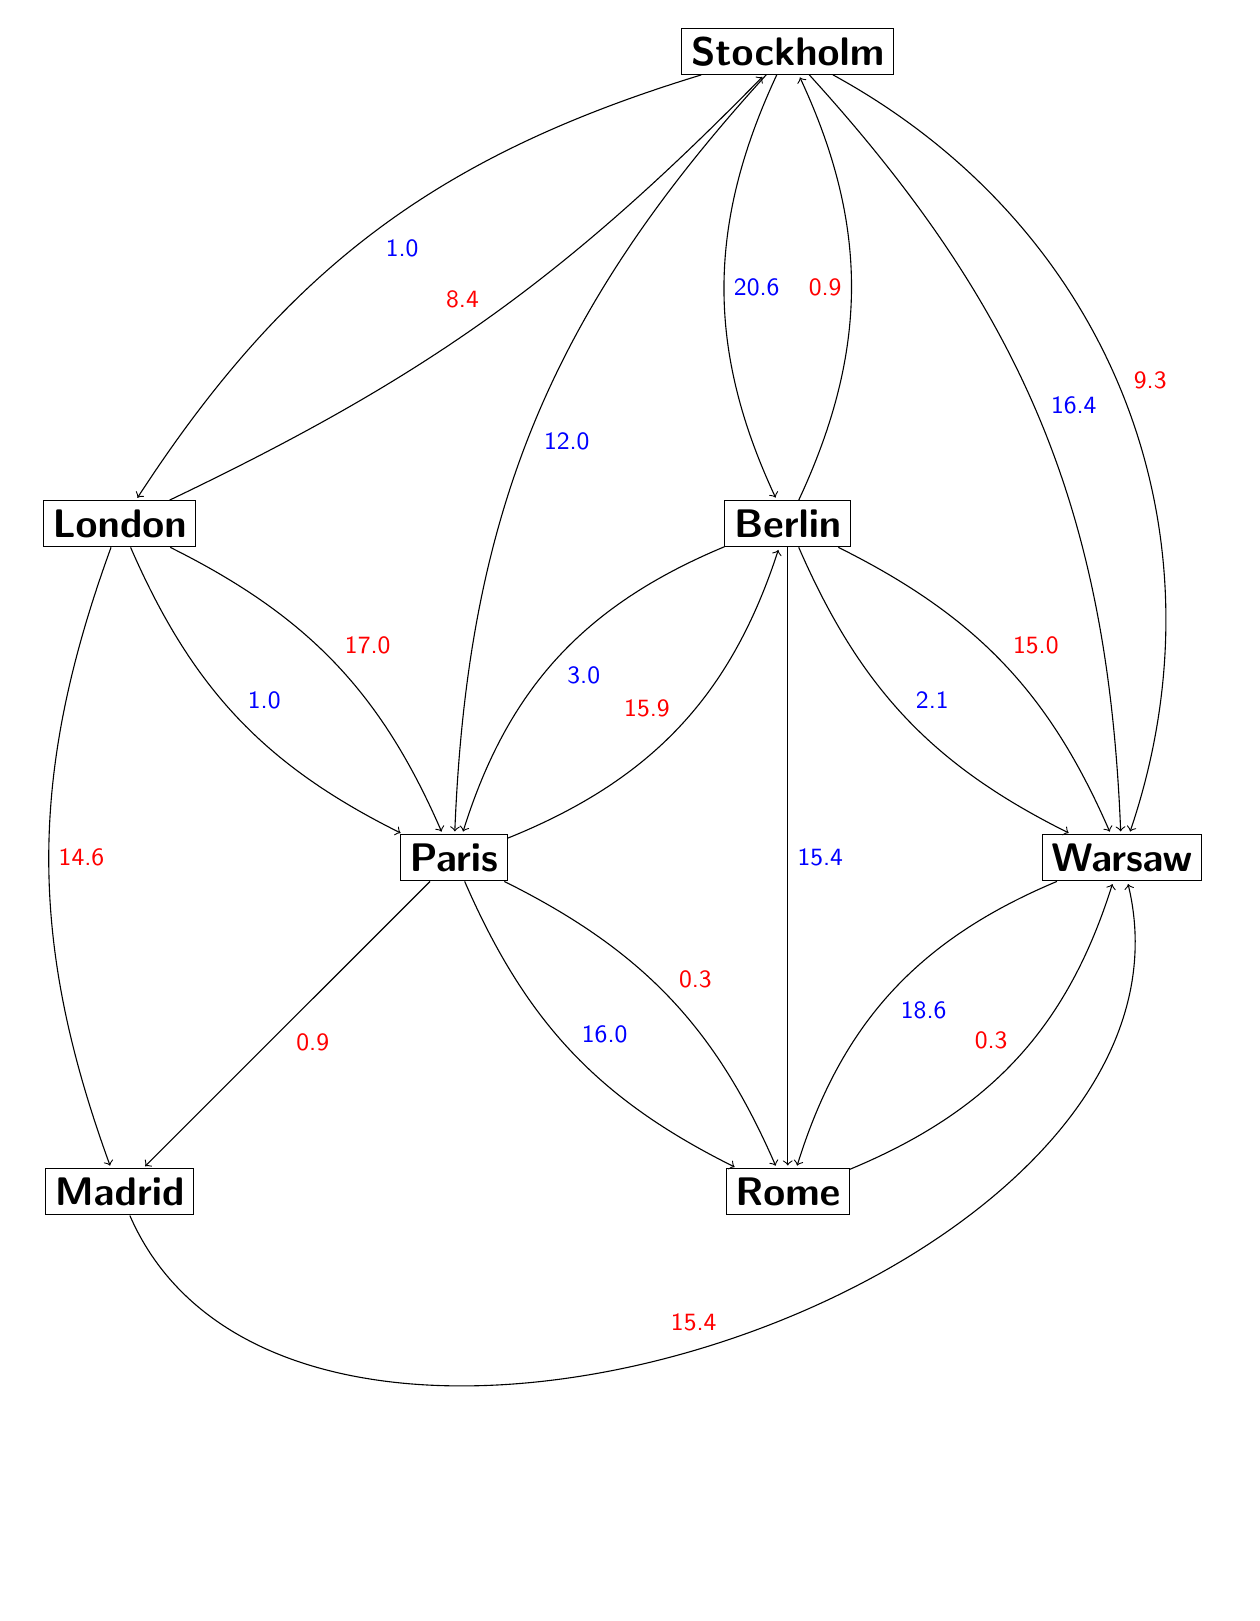
\begin{tikzpicture}[->,shorten >=1pt,auto,node distance=6cm,
                    main node/.style={rectangle,draw,font=\sffamily\Large\bfseries}]
  \node[main node] (1) {Stockholm};
  \node[main node] (2) [below of=1] {Berlin};
  \node[main node] (3) [below right of=2] {Warsaw};
  \node[main node] (4) [below left of=2] {Paris};
  \node[main node] (5) [above left of=4] {London};
  \node[main node] (6) [below right of=4] {Rome};
  \node[main node] (7) [below left of=4] {Madrid};

  \path[every node/.style={font=\sffamily\small}]
    (1) edge [bend right=20] node[blue] {1.0} (5)
    	edge [bend right=20] node[blue] {12.0} (4)
     	edge [bend right=25] node[blue] {20.6} (2)
    	edge [bend left=20] node[blue] {16.4} (3)
    	edge [bend left=40] node[red] {9.3} (3)
    (2) edge [bend right=25] node[red] {0.9} (1)
    	edge [bend right=25] node[blue] {3.0} (4)
        edge [bend right=20] node[blue] {2.1} (3)
    	edge [bend left=20] node[red] {15.0} (3)
    	edge node[blue] {15.4} (6)
    (3) edge [bend right=25] node[blue] {18.6} (6)
    (4) edge [bend right=25] node[red] {15.9} (2)
    	edge [bend right=20] node[blue] {16.0} (6)
    	edge [bend left=20] node[red] {0.3} (6)
    	edge node[red] {0.9} (7)
    (5) edge [bend right=10] node[red] {8.4} (1)
    	edge [bend left=20] node[red] {17.0} (4)
    	edge [bend right=20] node[blue] {1.0} (4)
		edge [bend right=20] node[red] {14.6} (7)
	(6) edge [bend right=25] node[red] {0.3} (3)
    (7) edge [bend right=85] node[red] {15.4} (3);
  
\end{tikzpicture}
\end{center}